%%%%%%%%%%%%%%%%%%%%%%%%%%%%%%%%%%%%%%%%%%%%%%%%%%%%%%%%%%%%%%%%%%%%%%
% Skupina20/main.tex -- Meja prepletenosti na procesorju IBM (stanja GHZ)
%
% Pravila predloge: brez \usepackage, slike v Skupina20/img/,
% vse oznake in ključi virov z "g20:", viri v ../references.bib.
%
% Besedilo v oglatih oklepajih [ ... ] je še za dopolniti.
% Okvirje "Opomba za skupino" pred oddajo IZBRIŠEMO.
%%%%%%%%%%%%%%%%%%%%%%%%%%%%%%%%%%%%%%%%%%%%%%%%%%%%%%%%%%%%%%%%%%%%%%

\graphicspath{{Skupina20/img/}}

\title{Meja prepletenosti na procesorju IBM: koliko kubitov lahko zares prepletemo v stanje GHZ?}
\titlerunning{Meja prepletenosti na procesorju IBM}
\author{[Ime Priimek], [Ime Priimek], [Ime Priimek] in [Ime Priimek]}
\maketitle

\abstract{[Povzetek napišemo na koncu, ko imamo rezultate. Vsebovati mora: raziskovalno vprašanje (največje število kubitov $N_{\max}$, ki jih procesor IBM Heron prepleta v stanje GHZ z zvestobo $F>0{,}5$), metodo (populacije in paritetne oscilacije, linearna veriga proti drevesu, dinamično razklapljanje in ublažitev napak branja), glavni rezultat s številko, npr.\ \enquote{Linearna veriga doseže $N_{\max}=[\ ]$, drevo z ublažitvijo pa $N_{\max}=[\ ]$}, in en stavek o pomenu.]}


%======================================================================
\begin{svgraybox}
\textbf{Opomba za skupino (pred oddajo izbriši).} To poglavje je ogrodje, ki ga skupaj dopolnjujemo. Uvod in Metode so že
napisani tako, da iz njih razberete, \emph{kaj} bomo merili in \emph{zakaj}; Rezultati, Razprava in Zaključek so še prazni.
Pred začetkom preberite:
\begin{itemize}
\item razdelek~\ref{g20:sec:uvod} (kaj je stanje GHZ in zakaj je $F>0{,}5$ prava meja),
\item razdelek~\ref{g20:sec:merjenje} (kako $F$ izmerimo -- to je jedro naloge),
\item razdelek~\ref{g20:sec:cas} (procesorski čas je omejen na 600~s v 28 dneh, zato \textbf{nič ne poženemo na pravem procesorju brez dogovora}).
\end{itemize}
Koda je v \texttt{koda/}, surovi rezultati z job ID v \texttt{rezultati/naloge.jsonl}. Roki: prijava teme 15.\,11.\,2026,
oddaja 22.\,11.\,2026, zagovor v tednu od 23.\,11.\,2026. Poročilo naj ima $\approx$\,10 strani.
\end{svgraybox}
%======================================================================


\section{Uvod}
\label{g20:sec:uvod}

Prepletenost je vir, ki kvantnim računalnikom omogoča prednost pred klasičnimi~\cite{nielsen2010}. Algoritmi, ki naj bi bili
uporabni, potrebujejo prepletenost čez veliko kubitov hkrati, današnji procesorji pa so šumni~\cite{preskill2018}: vsaka
dvokubitna vrata, vsak čas mirovanja in vsako branje prispevajo napako. Zato je naravno vprašanje, \emph{čez koliko kubitov
lahko danes dejansko ustvarimo prepletenost}. Na to vprašanje odgovarja priprava stanja Greenberger--Horne--Zeilinger
(GHZ)~\cite{g20:greenberger1990}
\begin{equation}
\ket{\mathrm{GHZ}_N} = \frac{1}{\sqrt{2}}\left(\ket{0}^{\otimes N} + \ket{1}^{\otimes N}\right),
\label{g20:eq:ghz}
\end{equation}
ki je \enquote{najbolj krhko} večdelno prepleteno stanje: ena sama napaka faze na kateremkoli kubitu uniči koherenco med
obema členoma. Stanje GHZ je zato strog in pogosto uporabljen preizkus kakovosti procesorja.

Mera, ki jo uporabimo, je zvestoba $F=\bra{\mathrm{GHZ}_N}\rho\ket{\mathrm{GHZ}_N}$ izmerjenega stanja $\rho$ glede na
idealno. Če velja $F>0{,}5$, je stanje dokazano \emph{pravo večdelno prepleteno} (angl.\ \emph{genuine multipartite
entanglement}), tj.\ ni ga mogoče zapisati kot mešanico stanj, v katerih bi bila katerakoli skupina kubitov ločena od
ostalih~\cite{g20:guhne2009}. Meja $0{,}5$ torej ni dogovor, ampak ima fizikalni pomen.

\textbf{Kaj so drugi že naredili.} Zvestobo stanj GHZ iz populacij in paritetnih oscilacij so prvič merili na ionih
(4~ioni~\cite{g20:sackett2000}, 14~ionov~\cite{g20:monz2011}). Na superprevodnih procesorjih IBM so poročali o 18-kubitnem
stanju z $F=0{,}517$~\cite{g20:wei2020} in o 27-kubitnem stanju z $F=0{,}546$ ob ublažitvi napak branja~\cite{g20:mooney2021}.
Leta 2025 je IBM z naprednimi tehnikami (prilagodljivo prevajanje, zaznavanje napak, začasno razračunavanje) pripravil
120-kubitno stanje GHZ z $F=0{,}56$~\cite{g20:ibm2025bigcats}. Pri predmetu NPMP v letih 2017/18--2025/26 nobena
seminarska naloga ni merila prepletenosti, ublažitve napak ali dinamičnega razklapljanja na realnem procesorju; skoraj vse so
implementacije znanih algoritmov.

\textbf{Kaj ostaja odprto.} Objavljeni rekordi uporabljajo tehnike in procesorski čas, ki jih študent z brezplačnim
paketom IBM Quantum Open Plan nima. Zanima nas, \emph{koliko daleč pridemo z vezji in ublažitvijo, ki so dostopni vsakomur}, in
kateri od teh vzvodov meji najbolj pomaga.

\begin{svgraybox}
\textbf{Raziskovalno vprašanje.} Koliko kubitov $N_{\max}$ lahko procesor IBM Heron (ibm\_fez, 156 kubitov) pripravi v stanje
GHZ z zvestobo $F>0{,}5$ in za koliko kubitov to mejo premakneta (a)~zasnova vezja (linearna veriga proti drevesu z majhno
globino) ter (b)~dinamično razklapljanje in ublažitev napak branja?

\textbf{Pričakovani rezultat.} Linearna veriga brez ublažitve doseže $N_{\max}\approx 15$--$20$. Drevo, prilagojeno
povezavam čipa, mejo vsaj podvoji, dinamično razklapljanje in ublažitev branja pa dodata še vsaj 20~\%; za najboljšo
kombinacijo pričakujemo $N_{\max}\approx 35$--$50$.
\end{svgraybox}

V razdelku~\ref{g20:sec:metode} opišemo vezja, način merjenja zvestobe in porabo procesorskega časa,
v razdelku~\ref{g20:sec:rezultati} rezultate na simulatorjih in procesorju, v razdelku~\ref{g20:sec:razprava} pa odgovorimo
na raziskovalno vprašanje in opišemo omejitve.


\section{Metode}
\label{g20:sec:metode}

\subsection{Orodja in nastavitve}
\label{g20:sec:orodja}

Vezja gradimo in izvajamo v okolju Qiskit~\cite{qiskit2024}, ker neposredno podpira procesorje IBM, njihove šumne modele in
dinamično razklapljanje. Različice in nastavitve so v tabeli~\ref{g20:tab:orodja}.

\begin{table}[htbp]
\caption{Orodja in nastavitve. [Dopolni ob glavnem zagonu.]}
\label{g20:tab:orodja}
\centering
\begin{tabular}{ll}
\toprule
Parameter & Vrednost \\
\midrule
Qiskit & 2.6.1 \\
Qiskit Aer & 0.18.2 \\
qiskit-ibm-runtime & 0.51.0 \\
ublažitev napak branja & mthree (M3)~\cite{g20:nation2021}, [različica] \\
kvantni procesor & ibm\_fez (IBM Heron, 156 kubitov) \\
šumni model & FakeFez (Qiskit) \\
primitiv & SamplerV2 \\
prevajanje & \texttt{optimization\_level=1}, [ročna postavitev kubitov] \\
dinamično razklapljanje & [XY4], [nastavitve] \\
število posnetkov (\emph{shots}) & 1000 na vezje \\
\bottomrule
\end{tabular}
\end{table}

\subsection{Vezja za pripravo stanja GHZ}
\label{g20:sec:vezja}

Stanje~\eqref{g20:eq:ghz} pripravimo z Hadamardovimi vrati na prvem kubitu in $N-1$ vrati CNOT, ki \enquote{širijo}
superpozicijo na ostale kubite. Število dvokubitnih vrat je pri obeh zasnovah enako ($N-1$), razlikuje pa se globina:

\begin{itemize}
\item \textbf{Linearna veriga} (slika~\ref{g20:fig:veriga}): CNOT-i si sledijo eden za drugim po poti kubitov na čipu.
      Globina raste kot $N$, zato prvi kubiti dolgo mirujejo in medtem dekoherirajo.
\item \textbf{Drevo} (slika~\ref{g20:fig:drevo}): vsak že prepleten kubit v naslednjem koraku prepleta svojega soseda, zato
      se število prepletenih kubitov v vsakem koraku lahko podvoji. Pri povezavah vsak-z-vsakim bi bila globina
      $\lceil\log_2 N\rceil$. Na procesorjih IBM so kubiti povezani v mrežo \emph{heavy-hex} (vsak kubit ima največ 3 sosede),
      zato drevo zgradimo z iskanjem v širino (BFS) iz osrednjega kubita; globina je tedaj sorazmerna z razdaljo do
      najbolj oddaljenega kubita, približno $\sqrt{N}$.
\end{itemize}
Obe vezji gradimo neposredno na grafu povezav procesorja, tako da prevajalnik ne doda vrat SWAP. Za vsako vezje poročamo
globino in število dvokubitnih vrat pred prevajanjem in po njem.

\begin{figure}[htbp]
\centering
\begin{subfigure}[b]{0.48\textwidth}
\centering
\begin{quantikz}[row sep=0.25cm, column sep=0.25cm]
\lstick{$q_0$} & \gate{H} & \ctrl{1} & \qw      & \qw      & \qw \\
\lstick{$q_1$} & \qw      & \targ{}  & \ctrl{1} & \qw      & \qw \\
\lstick{$q_2$} & \qw      & \qw      & \targ{}  & \ctrl{1} & \qw \\
\lstick{$q_3$} & \qw      & \qw      & \qw      & \targ{}  & \qw
\end{quantikz}
\caption{Linearna veriga, globina $N$.}
\label{g20:fig:veriga}
\end{subfigure}
\hfill
\begin{subfigure}[b]{0.48\textwidth}
\centering
\begin{quantikz}[row sep=0.25cm, column sep=0.25cm]
\lstick{$q_2$} & \qw      & \qw      & \targ{}   & \qw \\
\lstick{$q_0$} & \gate{H} & \ctrl{1} & \ctrl{-1} & \qw \\
\lstick{$q_1$} & \qw      & \targ{}  & \ctrl{1}  & \qw \\
\lstick{$q_3$} & \qw      & \qw      & \targ{}   & \qw
\end{quantikz}
\caption{Drevo, globina $\approx\log_2 N$.}
\label{g20:fig:drevo}
\end{subfigure}
\caption{Priprava 4-kubitnega stanja GHZ z dvema zasnovama vezja. V drevesu se zadnja CNOT-a izvedeta hkrati, zato je
vezje za en korak plitvejše; pri večjih $N$ razlika hitro raste. [Kasneje dodamo izris dejanske postavitve kubitov na ibm\_fez.]}
\label{g20:fig:vezja}
\end{figure}

\subsection{Merjenje zvestobe}
\label{g20:sec:merjenje}

Zvestobe ne moremo izmeriti z eno samo meritvijo. Za stanje GHZ jo razstavimo na dva dela, ki ju izmerimo ločeno~\cite{g20:sackett2000, g20:mooney2021}:
\begin{equation}
F = \frac{P + C}{2}.
\label{g20:eq:zvestoba}
\end{equation}

\textbf{Populacija $P$.} Vse kubite izmerimo v računski bazi; $P=p(0\dots0)+p(1\dots1)$ je delež posnetkov, ki dajo enega
od obeh pravilnih izidov. Idealno je $P=1$. Visok $P$ še ne pomeni prepletenosti -- enak $P$ bi dala tudi klasična mešanica
\enquote{vse 0 ali vse 1}.

\textbf{Koherenca $C$ (paritetne oscilacije).} Pred meritvijo na vsak kubit apliciramo rotacijo, ki ga meri v bazi
$\cos\phi\,X+\sin\phi\,Y$, in izračunamo pariteto $\Pi=\expval{Z^{\otimes N}}$ (delež sodih minus delež lihih izidov). Za
stanje GHZ velja
\begin{equation}
\expval{\Pi(\phi)} = C\cos(N\phi + \phi_0),
\label{g20:eq:pariteta}
\end{equation}
kjer je amplituda $C$ ravno velikost koherence med $\ket{0\dots0}$ in $\ket{1\dots1}$; idealno $C=1$, pri klasični mešanici
$C=0$. Pariteto izmerimo pri 16 enakomerno razporejenih vrednostih $\phi$ in $C$ določimo s prilagajanjem
enačbe~\eqref{g20:eq:pariteta} z znano frekvenco $N$.

\textbf{Negotovost in kriterij.} Negotovost $F$ ocenimo z zankanjem (angl.\ \emph{bootstrap}) po posnetkih. Za vsako
konfiguracijo je $N_{\max}$ največji $N$, pri katerem je $F-2\sigma_F>0{,}5$.

\subsection{Ublažitev napak}
\label{g20:sec:ublazitev}

\textbf{Dinamično razklapljanje (DD).} V času, ko kubit čaka, nanj apliciramo zaporedje pulzov (npr.\ XY4), katerih skupni
učinek je identiteta, vendar sproti izničijo počasno fazno napako zaradi okolice~\cite{g20:viola1999, g20:ezzell2023}. To
naj bi posebej pomagalo linearni verigi, kjer kubiti dolgo mirujejo.

\textbf{Ublažitev napak branja (M3).} Z dodatnimi kalibracijskimi vezji izmerimo, kako pogosto procesor prebere 0 kot 1 in
obratno, ter porazdelitev izidov popravimo~\cite{g20:nation2021}. Ker je to naknadna obdelava, ne potrebuje novih zagonov
glavnih vezij, samo kalibracijska vezja.

\subsection{Zasnova poskusov}
\label{g20:sec:poskusi}

\begin{enumerate}
\item \textbf{Idealni simulator} (Qiskit Aer): preverimo, da vezja in analiza dajo $F=1$ za vse $N$.
\item \textbf{Šumni model} FakeFez: celoten poskus brez porabe procesorskega časa; napoved $N_{\max}$.
\item \textbf{Pilotni zagon} na ibm\_fez: 1~posel, 20~vezij; preverimo časovni model in delovanje DD.
\item \textbf{Glavni zagon}: 4 konfiguracije (veriga/drevo $\times$ brez/z DD) $\times$ 8 velikosti
      $N\in\{5,10,15,20,25,30,40,50\}$ $\times$ 17 vezij (1 populacijsko + 16 paritetnih) + kalibracijska vezja M3.
\item \textbf{Ponovitev} najboljše konfiguracije na drugem procesorju (ibm\_kingston), da ocenimo, koliko je rezultat
      odvisen od posameznega čipa.
\end{enumerate}

\subsection{Poraba procesorskega časa}
\label{g20:sec:cas}

Paket Open Plan omogoča 600~s procesorskega časa v drsečem 28-dnevnem oknu. IBM porabo ocenjuje kot~\cite{g20:ibmjobtime}
\begin{equation}
t \approx 2\,\mathrm{s}\cdot n_\text{poslov} + 0{,}35\,\mathrm{ms}\cdot n_\text{vezij}\cdot n_\text{posnetkov},
\label{g20:eq:cas}
\end{equation}
kar se ujema s prvim zagonom (1 vezje $\times$ 1000 posnetkov: ocena 2,27~s, zaračunano 2~s). Ker je fiksni strošek posla
velik, vezja združujemo v malo poslov. Načrtovana poraba je v tabeli~\ref{g20:tab:cas}.

\begin{table}[htbp]
\caption{Načrtovana poraba procesorskega časa po enačbi~\eqref{g20:eq:cas}. [Dopolni z dejansko porabo, \texttt{job.usage()}.]}
\label{g20:tab:cas}
\centering
\begin{tabular}{lrrrr}
\toprule
Del poskusa & vezja & posli & ocena [s] & dejansko [s] \\
\midrule
prvi preizkus (5 kubitov) & 1 & 1 & 2,3 & 2 \\
pilotni zagon & 20 & 1 & 9 & [ ] \\
glavni zagon & 576 & 8 & 218 & [ ] \\
ponovitev na ibm\_kingston & 144 & 2 & 54 & [ ] \\
\midrule
skupaj & 741 & 12 & 283 & [ ] \\
\bottomrule
\end{tabular}
\end{table}

\subsection{Metrike}
\label{g20:sec:metrike}

\begin{itemize}
\item zvestoba $F$, populacija $P$ in koherenca $C$ v odvisnosti od $N$ (enačbi~\eqref{g20:eq:zvestoba} in~\eqref{g20:eq:pariteta}),
\item $N_{\max}$ za vsako konfiguracijo in prirastek $\Delta N_{\max}$ zaradi zasnove vezja oziroma ublažitve,
\item globina vezja, število dvokubitnih vrat in trajanje vezja pred prevajanjem in po njem,
\item porabljen procesorski čas na konfiguracijo.
\end{itemize}


\section{Rezultati}
\label{g20:sec:rezultati}

\textbf{Prvi preizkus na procesorju.} 2.\,11.\,2026 smo na ibm\_fez pognali 5-kubitno linearno verigo
(1000 posnetkov, job ID \texttt{dbk48fl6p51s73clupeg}). Po prevajanju je imelo vezje globino 20 in 4 vrata CZ. Porazdelitev
izidov je na sliki~\ref{g20:fig:ghz5}: $P = 0{,}460 + 0{,}395 = 0{,}855$. Asimetrija med $\ket{00000}$ in $\ket{11111}$ je
pričakovana, ker se kubit v stanju $\ket{1}$ med čakanjem na branje lahko sprosti v $\ket{0}$. Koherence $C$ v tem preizkusu
še nismo merili, zato zvestobe še ne poznamo.

\begin{figure}[htbp]
\centering
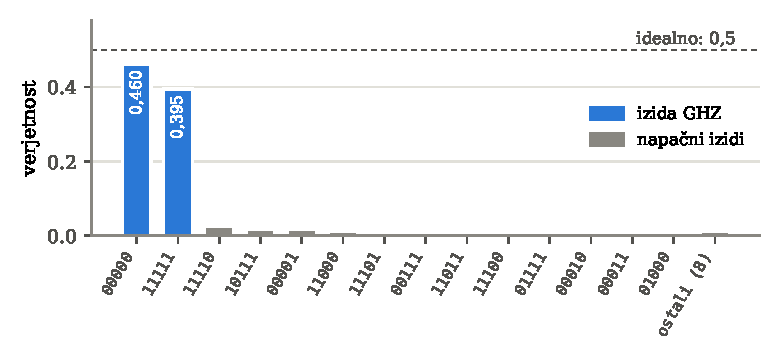
\includegraphics[width=0.85\textwidth]{ghz5_ibm}
\caption{Porazdelitev izidov 5-kubitnega stanja GHZ na procesorju ibm\_fez (1000 posnetkov). Izidi z manj kot 5 zadetki so
združeni v stolpec \enquote{ostali}. Sliko izriše \texttt{koda/izris\_ghz5.py}.}
\label{g20:fig:ghz5}
\end{figure}

[Tukaj pridejo: (1) tabela lastnosti vezij za vse $N$ in obe zasnovi; (2) graf $F(N)$ za idealni simulator, FakeFez in
ibm\_fez, vse 4 konfiguracije, z vodoravno črto pri $F=0{,}5$; (3) tabela $N_{\max}$ po konfiguracijah;
(4) primerjava z objavami~\cite{g20:wei2020, g20:mooney2021, g20:ibm2025bigcats}.]


\section{Razprava}
\label{g20:sec:razprava}

[Odgovor na raziskovalno vprašanje: ali se je hipoteza potrdila? Kateri vzvod (zasnova vezja, DD, ublažitev branja) je meji
najbolj pomagal in zakaj? Kako dobro je šumni model FakeFez napovedal rezultat procesorja?]

\textbf{Omejitve.} [Npr.: kalibracija procesorja se med dnevi spreminja; omejen procesorski čas dovoljuje le eno
ponovitev; ublažitev branja popravi branje, ne pa napak med pripravo stanja.]

\subsection{Kaj ni delovalo}
\label{g20:sec:neuspehi}

[Opišemo vsaj en neuspešen poskus in razlog. Kandidat že zdaj: naša skripta za preverjanje dostopa (\texttt{koda/preveri\_ibm.py}) je po prvem zagonu izpisala
porabo 0~s, ker je porabo prebrala, preden jo je IBM obračunal; dejanska poraba je bila 2~s.]


\section{Zaključek}
\label{g20:sec:zakljucek}

[Glavni rezultat v nekaj stavkih in predlog nadaljnjega dela, npr.\ dinamična vezja z meritvami sredi vezja, ki omogočajo
pripravo GHZ v konstantni globini.]


\section*{Doprinosi avtorjev}

[Za vsakega člana dva do tri stavke. Dogovorjena razdelitev:
\textbf{[Član 1]} -- gradnja vezij (veriga, BFS drevo) in izbira kubitov na čipu, razdelek Metode;
\textbf{[Član 2]} -- simulacije in zagoni na IBM, beleženje job ID in porabe časa;
\textbf{[Član 3]} -- analiza ($P$, $C$, $F$, bootstrap, M3) in grafi, razdelek Rezultati;
\textbf{[Član 4]} -- literatura, uvod, razprava, prosojnice in README.]

\section*{Izjava o uporabi generativne umetne inteligence}

[Pri pripravi naloge smo uporabili orodje generativne umetne inteligence za pregled tem prejšnjih let, pomoč pri pisanju kode za dostop do
IBM Quantum, osnutek predloga teme in ogrodja tega poglavja. Vse rezultate in besedilo smo preverili sami. Dopolni z
ostalimi orodji in nameni.]
